\documentclass{beamer}
\usetheme{Copenhagen}
\usecolortheme{orchid}
\title{CacaoScript: Syntax and Semantics}
\subtitle{A simple language for distributed applications on CacaoWeb}
\author{Ivan Chollet,Lucius Gregory Meredith,Paul Steckler}
\date{\today}

\AtBeginSection[]
{
  \begin{frame}
    \frametitle{ToC}
    \tableofcontents[currentsection]
  \end{frame}
}

\begin{document}
  \frame{\titlepage}
  \section{Overview}
  \section{Syntax}
  \begin{frame}
    \frametitle{Syntax}
    \begin{itemize}
      \item Core language is a mini-OCaml
      \item with sugar for
        \begin{itemize}
          \item Comprehensions
          \item Delimited continuations
          \item Reflection (quote and unquote)
        \end{itemize}
    \end{itemize}
  \end{frame}
  \subsection{Core language}
  \begin{frame}
    \frametitle{Core language I}
    \begin{figure}[ht]
      \begin{center}        
        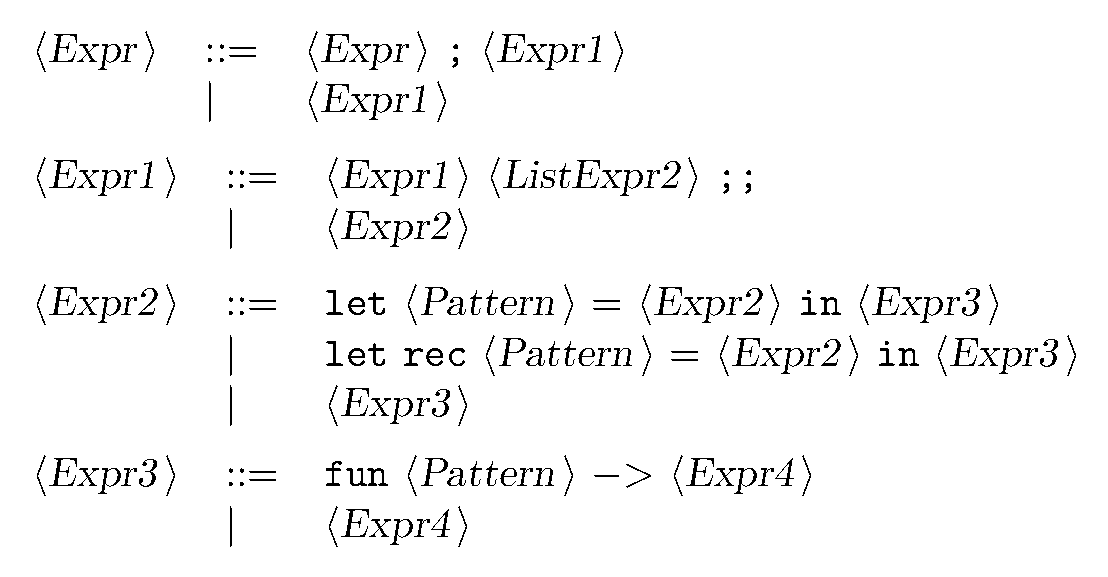
\includegraphics[height=2in]{pipelinefigures/CoreLanguageSyntaxI.pdf}
      \end{center}      
    \end{figure}
  \end{frame}
  \begin{frame}
    \frametitle{Core language II}
    \begin{figure}[ht]
      \begin{center}        
        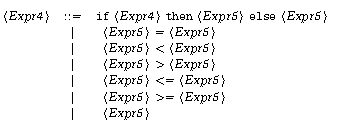
\includegraphics[width=\textwidth,height=0.8\textheight,keepaspectratio]{pipelinefigures/CoreLanguageSyntaxII.pdf}
      \end{center}      
    \end{figure}
  \end{frame}
  \begin{frame}
    \frametitle{Core language III}
    \begin{figure}[ht]
      \begin{center}        
        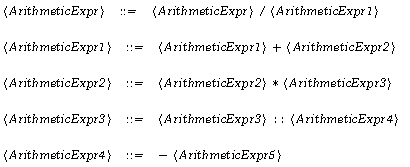
\includegraphics[width=\textwidth,height=0.8\textheight,keepaspectratio]{pipelinefigures/CoreLanguageSyntaxIII.pdf}
      \end{center}      
    \end{figure}
  \end{frame}
  \subsection{Sugar}
  \subsubsection{Comprehensions}
  \begin{frame}
    \frametitle{Comprehensions}
    \begin{figure}[ht]
      \begin{center}        
        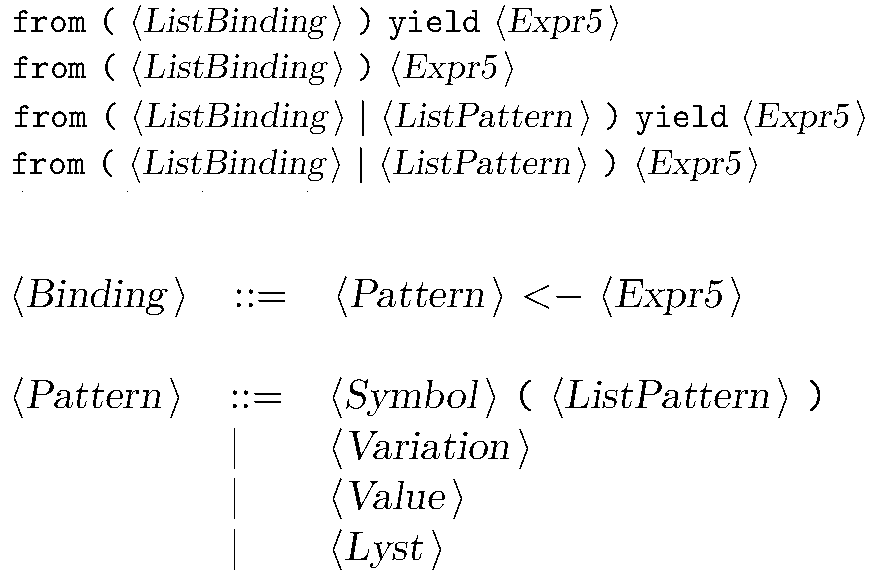
\includegraphics[height=2in]{pipelinefigures/SyntaxSugarComprehensions.pdf}
      \end{center}      
    \end{figure}
  \end{frame}
  \subsubsection{Delimited continuations}
  \begin{frame}
    \frametitle{Delimited continuations}
    \begin{figure}[ht]
      \begin{center}        
        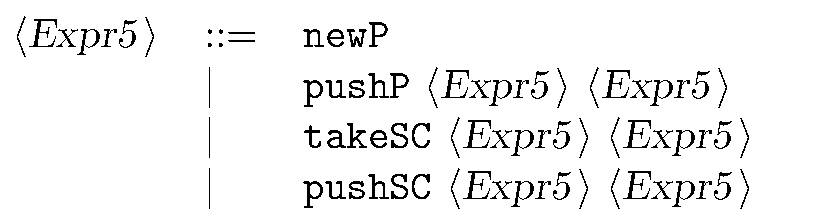
\includegraphics[width=\textwidth,height=0.8\textheight,keepaspectratio]{pipelinefigures/SyntaxSugarDelimCC.pdf}
      \end{center}      
    \end{figure}
  \end{frame}
  \subsubsection{Reflection}
  \begin{frame}
    \frametitle{Reflection}
  \end{frame}
  \section{Example programs}
  \begin{frame}
    \frametitle{Example programs}
    \begin{itemize}
      \item simple arithmetic
      \item obligatory lambda abstraction application example
      \item in-place update of a key-value map
      \item concurrency examples        
    \end{itemize}
  \end{frame}
  \subsection{The basics: arithmetic}
  \begin{frame}
    \frametitle{Sum, products, etc}    
  \end{frame}
  \subsection{The basics: abstraction and application}
  \begin{frame}
    \frametitle{$(\lambda x.x)(\lambda x.x)$}    
  \end{frame}
  \subsection{More realistic examples: in-place update of map}
  \begin{frame}
    \frametitle{in-place update with delimcc}    
    \begin{figure}[ht]
      \begin{center}        
        \includegraphics[height=2in]{pipelinefigures/InplaceUpdateCodeSampleI.pdf}
      \end{center}      
    \end{figure}
  \end{frame}
  \begin{frame}
    \frametitle{in-place update with delimcc}    
    \begin{figure}[ht]
      \begin{center}        
        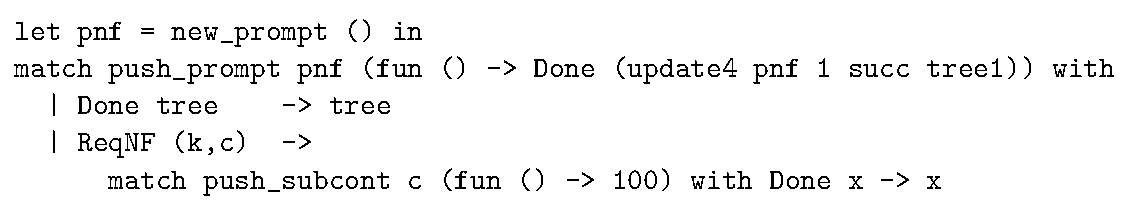
\includegraphics[width=\textwidth,height=0.8\textheight,keepaspectratio]{pipelinefigures/InplaceUpdateClientCode.pdf}
      \end{center}      
    \end{figure}
  \end{frame}
  \begin{frame}
    \frametitle{in-place update with delimcc}    
    \begin{figure}[ht]
      \begin{center}        
        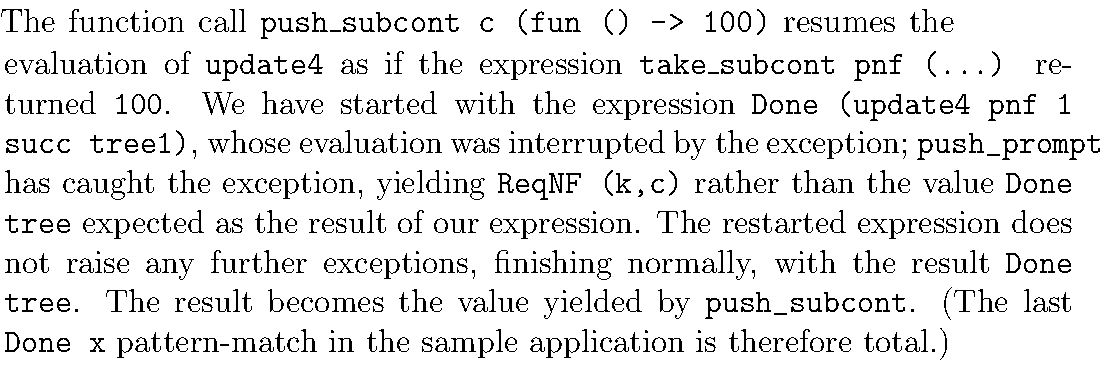
\includegraphics[width=\textwidth,height=0.8\textheight,keepaspectratio]{pipelinefigures/InplaceUpdateExplanation.pdf}
      \end{center}      
    \end{figure}
  \end{frame}
  \begin{frame}
    \frametitle{in-place update with delimcc}    
    \begin{figure}[ht]
      \begin{center}        
        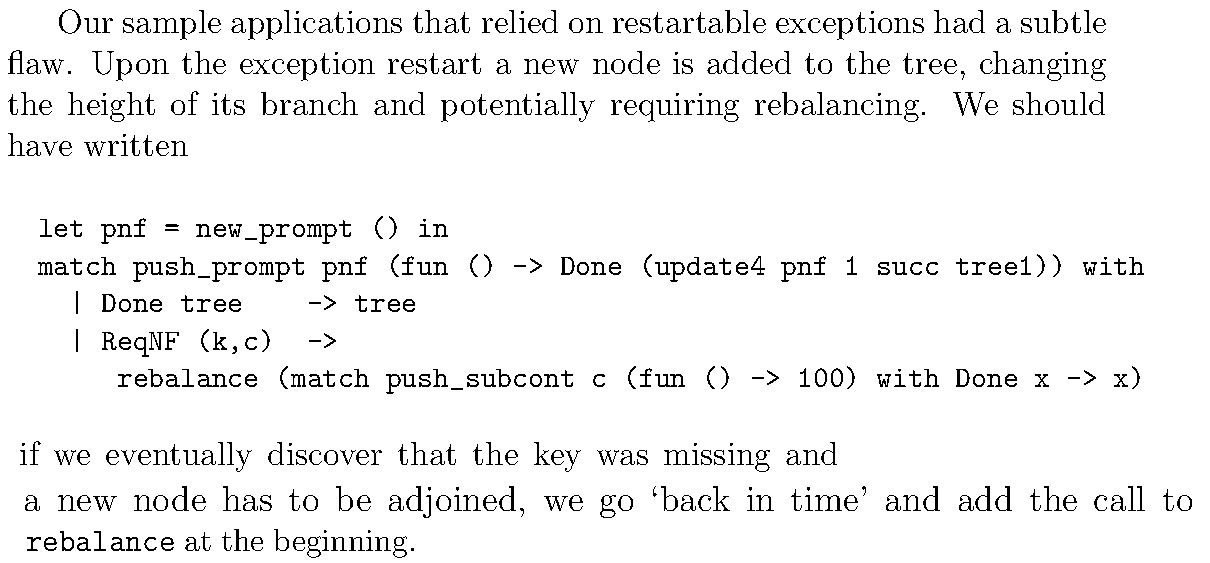
\includegraphics[width=\textwidth,height=0.7\textheight,keepaspectratio]{pipelinefigures/InplaceUpdateElaboration.pdf}
      \end{center}      
    \end{figure}
  \end{frame}
  \subsection{More realistic examples: concurrency}
  \begin{frame}
    \frametitle{concurrency}    
  \end{frame}
  \section{The pipeline}
  \begin{frame}
    \frametitle{The pipeline}
    \begin{figure}[ht]
      \begin{center}        
        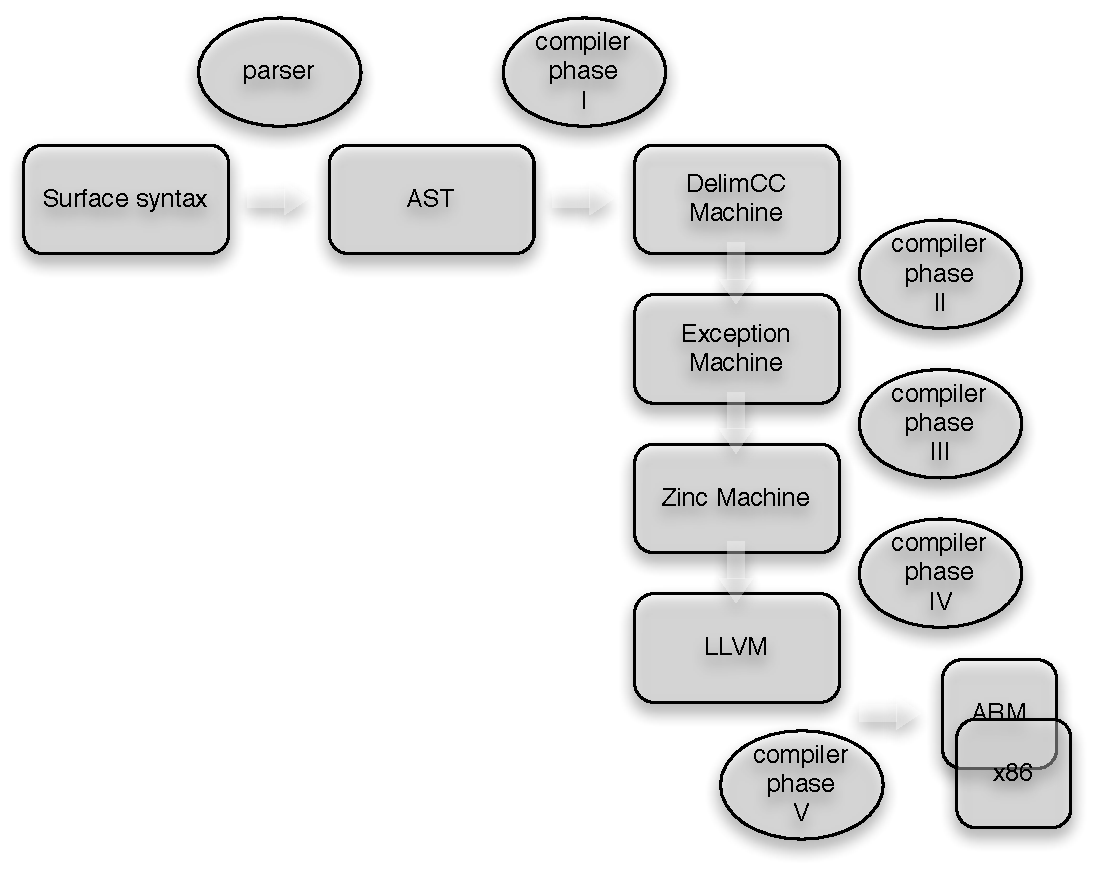
\includegraphics[height=2in]{pipelinefigures/PipelineImageI.pdf}
      \end{center}      
    \end{figure}
  \end{frame}
  \section{The delimCC machine}
  \begin{frame}
    \frametitle{The delimCC machine}
    \begin{figure}[ht]
      \begin{center}        
        \includegraphics[height=2in]{pipelinefigures/DelimCCMachineSpec1.svg/image1.pdf}
      \end{center}      
    \end{figure}

  \end{frame}
  \section{The exception machine}
  \begin{frame}
    \frametitle{The exception machine}
    \begin{figure}[ht]
      \begin{center}        
        \includegraphics[height=2in]{pipelinefigures/ExceptionMachineSpec1.svg/image2.pdf}
      \end{center}      
    \end{figure}
  \end{frame}
  \section{Eliminating the delimCC machine}
  \begin{frame}
    \frametitle{Eliminating the delimCC machine}
    \begin{figure}[ht]
      \begin{center}        
        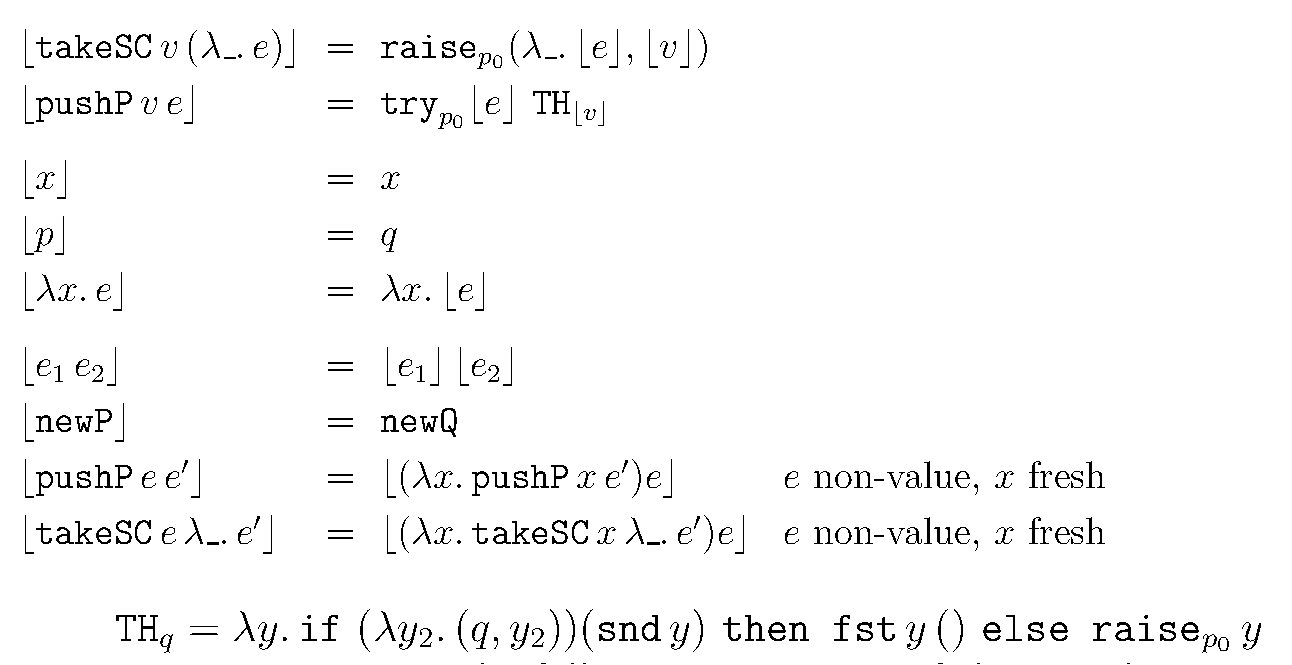
\includegraphics[height=2in]{pipelinefigures/EliminatingDelimCCMachine.pdf}
      \end{center}      
    \end{figure}

  \end{frame}
  \section{The Zinc machine}
  \begin{frame}
    \frametitle{The Zinc machine}
  \end{frame}
  \section{LLVM}
  \begin{frame}
    \frametitle{The LLVM}
  \end{frame}
  \section{Conclusions}
  \begin{frame}
    \frametitle{Conclusions}
  \end{frame}
\end{document}